\chapter{Microbially induced soil aggregate turnover across different climates and moisture regimes}
\label{chap:manuscript4} % Label for potential cross-referencing (start page)

\begin{center}
  \textbf{\Large Manuscript 4}
\end{center}  

\vspace{0.1cm}

\begin{center}
  \textbf{\huge Microbially induced soil aggregate turnover across different climates and moisture regimes}
\end{center}

\vspace{0.2cm}

\begin{center}
  \textit{Geoderma}\\
  \textit{DOI 10.2139/ssrn.4740477}
\end{center}

\vspace{0.1cm}

\begin{justify}
    Julia Mitzscherling\textsuperscript{1}, Rómulo Oses\textsuperscript{2}, Nicolás Riveras-Muñoz\textsuperscript{3}, Carsten W. Müller\textsuperscript{4,5}, Oscar Seguel\textsuperscript{6},   Peter Kühn\textsuperscript{3}, Thomas Scholten\textsuperscript{3} and Dirk Wagner\textsuperscript{1,7}
\end{justify}

  \vspace{0.2cm}
  
  \begin{scriptsize}
    \begin{justify}
        
      \textsuperscript{1}GFZ German Research Centre for Geosciences, Section Geomicrobiology, Telegrafenberg D-14473 Potsdam, Germany\\
      \textsuperscript{2}Centro Regional de Investigaci{\'o}n y Desarrollo Sustentable de Atacama, Universidad de Atacama (CRIDESAT UDA), Copayapu 484, Copiap{\'o}, Chile\\
      \textsuperscript{3}University of T{\"u}bingen, Soil Science and Geomorphology, R{\"u}melinstrasse 19--23, D-72070 T{\"u}bingen, Germany\\
      \textsuperscript{4}Institute of Ecology, Chair of Soil Science, Technische Universit{\"a}t Berlin, 10587 Berlin, Germany\\
      \textsuperscript{5}Department of Geosciences and Natural Resource Management, University of Copenhagen, 1350 Copenhagen K, Denmark\\
      \textsuperscript{6}Universidad de Chile, Facultad de Ciencias Agron{\'o}micas, Av. Santa Rosa \#11315, La Pintana, 8820808 Santiago, Chile\\
      \textsuperscript{7}University of Potsdam, Institute of Geosciences, Karl-Liebknecht-Strasse 24--25, D-14476 Potsdam, Germany

    \end{justify}
  \end{scriptsize}
    
  \vspace{0.4cm}

  \begin{flushleft}
    Received: 27 February 2024
  \end{flushleft}
  \cleardoublepage

\section*{Abstract}

While it is widely recognized that soil structure stability is related to soil physical, chemical and biological processes and properties, the role of the types of microorganisms in this respect is still unclear. Particularly, knowledge on the relative roles of abiotic versus biotic mechanisms is scarce. Our study investigated the influence of microbial activity on soil aggregate development across diverse climatic settings under wetting-drying (W-D) cycles and constantly moist conditions. Further, we evaluated the response of prokaryotic communities and microbial abundance to changing soil moisture conditions. Analyses encompassed soils from arid, semi-arid, mediterranean, and humid climates. Findings reveal the pronounced impact of climate legacy on soil structure responses to climate variations. Variations in soil aggregate attributes and microbial communities, driven by pedogenesis and climatic conditions, dictate how soil aggregation and microbial communities respond to changing soil moisture levels. In arid soils, the Birch-effect stimulated microbial activity and led to the breakdown of larger aggregates via labile organic matter consumption. Semi-arid soils showed microbial-mediated microaggregate formation through organic matter decomposition, ultimately decreasing soil stability. In mediterranean soils, increased microbial activity facilitated microaggregate assembly from silt-clay fractions, enhancing soil stability despite reductions in larger aggregates. Humid soils displayed unique responses, with fungi significantly enhancing stability, and prokaryotic activity stimulated by W-D. Conversely, microbial abundance substantially declined under constant moisture due to moisture stress, albeit a noteworthy increase in soil stability. Understanding these microbial-soil interactions as affected by climate is crucial for understanding initial soil formation processes as well as sustainable soil management, offering insights into soil health and ecosystem resilience.

\section*{Keywords} % Use \section* for unnumbered sections if needed
Soil aggregation, soil formation, Illumina MiSeq, microbial key players, microbial communities, wetting-drying cycles, climate gradient

\section{Introduction}

Most of the Earth's surface comprises soils and sediments, profoundly shaping the landscape by resisting erosion, influenced by the action of water in various climate regimes. Research exploring the interplay between biotic and abiotic processes in ecosystems has investigated organism-mineral interactions \citep{Brehm2005, Quirk2012} and biotic activities inducing soil and landscape formation \citep{Dietrich2006}. Biota impact terrestrial surfaces through mineral weathering, ion formation, and biofilm generation, which may control erosion resistance to a large extent \citep{Gadd2010, Gorbushina2007, RiverasMunoz2022}. Although recognized early that soil stability relates to physical, chemical, and biological processes, the specific role of microorganisms remains unclear, lacking a comprehensive understanding of their mechanisms and species contributions in varied climate contexts.

Typically, soils exhibit a complex three-dimensional arrangement comprising aggregates interspersed with void spaces \citep{Bailey2013, Oades1991}, increasingly referred to as soil architecture \citep{Amelung2023}. Aggregates consist of clusters of mineral particles and organic carbon, wherein the internal forces binding the particles together within each aggregate are much stronger than the forces acting between neighboring aggregates \citep{Six2004}. This strength enables the structures to endure wetting events and mechanical disruptions within the bulk soil \citep{Bravo2018}. These aggregates assemble hierarchically forming networks of particles and voids that are periodically connected during wetting episodes, which in turn create a variable flow of water and nutrients, offering access to soil organisms \citep{Wilpiszeski2019}.

In general, soil aggregates are grouped according to their size. Microaggregates (\SI{< 250}{\micro\metre}) consist of clay particles, organo-mineral complexes, and polyvalent metals, bound by bacterial polysaccharides \citep{Six2004, Totsche2018}, while macroaggregates (\SI{> 250}{\micro\metre}) are formations of minerals and particulate organic matter (POM), and are mainly bound by fungal hyphae and plant roots \citep{Oades1984}.

Soil aggregation is highly correlated with soil moisture, clay and organic carbon content \citep{AlKaisi2014} and is one controlling factor of the dynamic and spatial variation in soil properties \citep{Totsche2018}. The moisture regime in soils is largely controlled by climate which in turn controls soil formation. This has been shown in great detail along the Coastal Cordillera of Chile \citep{Bernhard2018}. Climatic factors such as precipitation and temperature affect soil biological, soil chemical and soil physical processes such as the accumulation or organic carbon, weathering of minerals and swelling and shrinking of clay particles as well as soil properties. Terrestrial ecosystems experience regular changes in water availability, a critical resource for life. Alternating wet-dry events significantly influence soil aggregate formation and stabilization processes \citep{Najera2020}.

Additionally, microbial activity, i.e. the production of binding material such as exudates, and fungal hyphae affect aggregate formation \citep{Tisdall1982}, while soil aggregation also indirectly affects microbial activity as well as community structure \citep{Biesgen2020}. It has been shown that macro- and microaggregates are characterized by different predation pressure and, therefore, contain distinct microhabitats \citep{Fox2018, Mummey2004, Sessitsch2001}. Microbial residents occupy specialized niches within the aggregate structure, with active microorganisms living both within and between aggregate particles \citep{Bailey2013, Ebrahimi2016, Sessitsch2001}. The complex feedback between mineralogy and biology begins with the weathering of the parent material. It continues with the formation of aggregates and the stabilization of the microscale architecture of the soil structure and generally controls the geochemical cycles in the soil matrix during the development of a soil \citep{Crawford2012, Lynch1985}.

The influence of microorganisms on soil aggregate formation has been highlighted in several studies before \citep{Chotte2005, Gupta2015, Tisdall1982}. However, taxonomic groups driving the process and acting as potential key players are still largely unknown, while the mechanisms controlling the formation and persistence of soil aggregates are yet not fully understood. Particularly, knowledge of the relative roles of abiotic (water, organic-mineral-interactions) versus biotic (plant C input, microbial activity) drivers of aggregate formation is lacking. Therefore, we hypothesize that the abundance, diversity and composition of soil microbial communities are characteristic of different stages of soil development and as a corollary, that specific taxonomic groups are related to the distribution and stability of aggregates at each developmental stage.

Hence, this work aimed to (i) unveil the microbial contributions to soil aggregate formation and stabilization compared to abiotic processes in soils of different climatic conditions and developmental stages during repeated wetting-drying (WD) cycles, and (ii) identify microbial key players involved in aggregate formation and stabilization.

Since studies on the development of abiotic and biotic interactions are very complex, they require both different spatial and temporal scales \citep{Ollivier2011}. Therefore, soils were collected from four locations along the Coastal Cordillera of Chile representing a natural climate gradient, ranging from arid over semi-arid and mediterranean to humid conditions. In order to unveil the microbial role in the process of aggregate formation and stabilization, the manipulation of soil moisture by applying W-D cycles was performed with a set of native soils including the indigenous microbial communities and a set of sterilized soil samples without any microorganisms. Quantification of bacteria, archaea, and fungi by qPCR was used to document the response patterns of microbial abundances and communities. We performed Illumina MiSeq sequencing of 16S rRNA genes to gain a detailed picture of the microbial community structure and their shifts during W-D cycling. Changes in the microbial communities were related to edaphic parameters such as soil aggregate sizes, carbon and nitrogen content, C/N ratio and aggregate stability.

\section{Materials and methods}
\subsection{Field site description and sampling}

In the frame of the EarthShape project (German Science Foundation SPP 1803), soils were studied at the following four study sites distributed over \SI{1300}{\kilo\metre} along the Chilean Coastal Cordillera: Pan de Az{\'u}car National Park (\(\sim\)\ang{26}S), Santa Gracia Nature Reserve (\(\sim\)\ang{30}S), La Campana National Park (\(\sim\)\ang{33}S), and Nahuelbuta National Park (\(\sim\)\ang{38}S). The study sites cover a climate gradient with decreasing annual temperature and increasing annual precipitation from north to south and corresponded to arid, semi-arid, mediterranean and humid climates (\ref{fig:M4-F1}) resulting in different soil moisture regimes \citep{Bernhard2018}. Due to the long-term impact of stable climate conditions \citep{Ewing2006} soils show different stages of soil development. They were classified into Regosols in Pan de Az{\'u}car, Cambisols in Santa Gracia and La Campana, and Umbrisols in Nahuelbuta \citep{Bernhard2018}. Vegetation types range from very sparse higher plant desert vegetation in the north, where biocrust soil coverage can reach as much as \SI{40}{\percent} of the area (biocrust-dominated desert vegetation) over semi-desert open shrubland and mediterranean dry forest and to temperate mixed broadleaved-coniferous forest in the south \citep{Bernhard2018a, Bernhard2018}.

Surface depth increments (\SIrange{0}{5}{\centi\metre}) were collected in March--April 2016 on the mid slope position of the South-facing hillslopes in each study site and were directly sieved (\SI{< 2}{\milli\metre}) on ethanol-sterilized sieves to remove coarse organic material and stones. Samples were stored at \SI{4}{\degreeCelsius} until further processing. 
Detailed site-specific descriptions and soil classifications were performed by \citet{Bernhard2018a}, \citet{Bernhard2018} and \citet{Oeser2018a}, \citet{Oeser2018b}.

\begin{figure}[H]
	\centering
	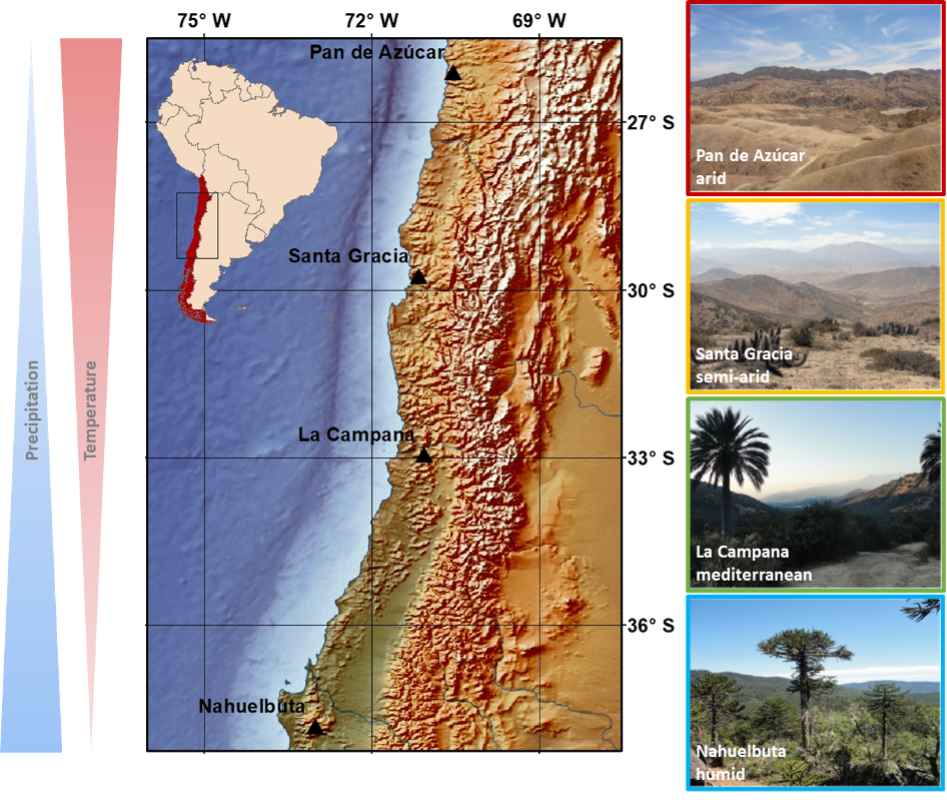
\includegraphics[width=1\textwidth]{img/M4-Figure_1.png}
	\caption{Location of the four study sites along the climate gradient on the Chilean Coastal Cordillera. MAP, mean annual precipitation; MAT, mean annual temperature.}
	\label{fig:M4-F1}
\end{figure}

\subsection{Experimental design}

Aggregate formation was developed during repeated W-D cycles using T{\"u}bingen cups (T-cup), which were covered by a fine silk cloth at the bottom \citep{Scholten2011}. In order to characterize the role of microorganisms on soil-structure formation processes, sets of soil samples with the indigenous microbial community (native) and sterilized control samples were prepared. The control samples were sterilized by cobalt-60 gamma-irradiation (SteriXpert, BBF Sterilisationsservice GmbH, Kernen-Rommelshausen, Germany). Each T-cup (\(h = \SI{5}{\centi\metre}\), \(r = \SI{2.5}{\centi\metre}\)) was filled with \SI{60}{\gram} soil material, followed by 22 days at \SI{22}{\degreeCelsius} to acclimate the soil-dwelling microorganisms to laboratory conditions. The manipulation experiment was performed by incubating the T-cups under controlled environmental conditions for a total time duration of six weeks. We saturated the soil to field capacity (pF 1.8, \SI{-60}{\hecto\pascal} pressure) at room temperature on a sterile sand bed (grain size \SIrange{0.06}{0.25}{\milli\metre}) for 24 hours. This was followed by a drying step at \SI{25}{\degreeCelsius} in an oven for 1--2 days until equilibrium. In addition, one sample remained on the sand bed throughout the entire experiment, being constantly subjected to moisture. Duplicate samples of native and sterilized soil material were collected after fulfilled cycles, comprising time point zero (R0), one, three, and six W-D cycles (R1, R3, R6), and after six weeks of constant moisture (CM). Separate T-cups were prepared for the different analytical approaches, one for DNA-based methods and one for the analysis of soil properties. Cups for DNA-analysis were stored at \SI{-20}{\degreeCelsius} and cups for the analysis of soil properties at \SI{4}{\degreeCelsius} until further processing.

\subsection{Soil properties, aggregate size distribution and stability}

Soil-chemical properties were analyzed for the native and the sterilized soils. The total organic carbon (TOC) was determined by Potsdamer Wasser- und Umweltlabor GmbH (PWU, Potsdam, Germany) according to DIN EN ISO/IEC 17025:2005. The aggregate size separation was done by wet sieving adapted from \citet{Elliott1986} as described in \citet{RiverasMunoz2022}. In the first step, \SI{10}{\gram} of soil material was irrigated with \SI{50}{\milli\liter} water. A series of four sieves, which were placed in descending order, was used to obtain the following soil aggregate size classes: (i) $>$\SI{500}{\micro\meter} (large macroaggregates); (ii) \SIrange{250}{500}{\micro\meter} (small macroaggregates); (iii) \SIrange{53}{250}{\micro\meter} (large microaggregates); (iv) \SIrange{20}{53}{\micro\meter} (small microaggregates), and (v) $<$\SI{20}{\micro\meter} (silt/clay).

Aggregates were separated manually by moving the sieve up and down 30 times during \SI{5}{\minute} in a \SI{2.5}{\liter} water tank. The aggregate classes retained on each sieve were oven-dried at \SI{105}{\degreeCelsius}, and weighed. In the following, large and small macroaggregates are referred to as macroaggregates (MAC), large and small microaggregates are referred to as microaggregates (MIC) and the silt/clay class is referred to as SC.

The mean weight diameter (MWD in \si{\milli\metre}), a measure of aggregate stability determined by the size distribution of aggregates \citep{Amezketa1999}, was calculated as an average weighed by aggregate size.

Furthermore, the soil organic carbon (SOC) and total nitrogen (TN) content of each aggregate size class was measured using oxidative heat combustion at \SI{1150}{\degreeCelsius} in a Vario EL III elemental analyzer (Elementar Analysensysteme GmbH, Hanau, Germany) and subsequently, the C/N ratio was calculated. SOC and total carbon were used interchangeably since the study sites showed low inorganic carbon content \citep{RiverasMunoz2022}.

\subsection{DNA extraction and quantification of bacteria, archaea, and fungi}

Total genomic DNA was extracted from the native soil material using the DNeasy\textsuperscript{\textregistered} PowerSoil\textsuperscript{\textregistered} Kit (Qiagen GmbH, Hilden, Germany) with a maximum amount of \SI{0.25}{\gram} per sample. DNA was extracted in triplicates following the manufacturer’s protocol with one exception: DNA elution was done with PCR-grade water. Final DNA concentrations were measured with a Qubit\textsuperscript{\textregistered} 2.0 Fluorometer using the Qubit\textsuperscript{TM} dsDNA HS Assay Kit (both Invitrogen Life Technologies, Thermo Fisher Scientific, Carlsbad CA, USA). DNA extracts were stored at \SI{-20}{\degreeCelsius} until further processing.

Gene copy numbers of bacteria, archaea, and fungi were determined by quantitative polymerase chain reaction (qPCR). 16S rRNA genes were amplified by using the bacterial primer pair Eub341F (5\('\)-\texttt{CCT ACG GGA GGC AGC AG}-3\('\)) and Eub534R (5\('\)-\texttt{ATT ACC G CG GCT GCT GG}-3\('\)) \citep{Muyzer1993} and the archaeal primer pair 340F (5\('\)-\texttt{CCC TAC GGG GYG CAS CAG}-3\('\)) and 1000R (5\('\)-\texttt{GGC CAT GCA CYW CYT CTC}-3\('\)) \citep{Gantner2011}. 28S rRNA genes were amplified by using the fungal primer pair NL1F (5\('\)-\texttt{ATA TCA AAT AAG CGG AGG AAA AG}-3\('\)) and LS2R (5\('\)-\texttt{ATT CCC AAA CAA CTC GAC TC}-3\('\)) \citep{Bates2009}. The qPCR assay was carried out in a total reaction volume of \SI{20}{\micro\liter} using the KAPA SYBR\textsuperscript{\textregistered} FAST qPCR Kit Master Mix (2x) Universal (Kapa Biosystems, Sigma-Aldrich, Germany). Quantification was performed in the CFX96 Connect\textsuperscript{TM} Real-Time System (Bio-Rad Laboratories, CA, USA) with the following cycling program for bacteria/ archaea/ fungi: initial denaturation at \SI{95}{\degreeCelsius} for \SI{3}{\minute}, followed by 40/ 45/ 45 cycles of denaturation at \SI{95}{\degreeCelsius} for \SI{3}{\second}, annealing at \SI{60}{\degreeCelsius}/ \SI{57}{\degreeCelsius}/ \SI{50}{\degreeCelsius} for \SI{20}{\second}, and elongation at \SI{72}{\degreeCelsius} for \SI{30}{\second}. Fluorescence was measured at \SI{80}{\degreeCelsius}. The melting curve was recorded by rising temperature from \SI{65}{\degreeCelsius} to \SI{95}{\degreeCelsius}. DNA extracts from Pan de Az{\'u}car were added undiluted, samples from La Campana and Santa Gracia were used in 1:100 dilutions, as well as samples from Nahuelbuta with one exception: constant moisture samples were used in 1:10 dilutions. Every qPCR run included blanks, calibration standards, and soil samples in triplicates. The reaction efficiency ranged between \SIrange{96.3}{103.9}{\percent}. Data were analyzed using the CFX Manager\textsuperscript{TM} Software (Bio-Rad Laboratories, CA, USA).

\subsection{Illumina MiSeq amplicon sequencing of bacteria and archaea}

PCR products were prepared for Illumina MiSeq high-throughput sequencing of bacterial and archaeal 16S rRNA genes. Unique primer combinations of barcode tagged 515F (5\('\)-\texttt{GTG CCA GCM GCC GCG GTA A}-3\('\)) and 806R (5\('\)-\texttt{GGA CTA CGV GGG TWT CTA AT}-3\('\)) primers were assigned to each sample \citep{Caporaso2012}. For each genomic DNA sample, two technical replicates with different barcodes were amplified by PCR and sequenced. For a detailed description of the library preparation, the reader is referred to \citet{Moskwa2020}.

\subsection{Bioinformatics and statistical analysis}

Sequencing was performed at Eurofins Genomics (Konstanz, Germany) on an Illumina MiSeq generating \(2\times 300\)\,bp paired-end reads. The sequencing library was demultiplexed using \texttt{cutadapt} v3.4 \citep{Martin2011} using the following parameters: \texttt{-e 0.2 -q 15,15 -m 150 --discard-untrimmed}. The ASVs were generated using trimmed reads and the \texttt{DADA2} package v1.20 \citep{Callahan2016} with R v4.1 using the pooled approach with the following parameters: \texttt{truncLen=c(240,200), maxN=0, rm.phix=TRUE, minLen=200}. Taxonomic assignment was done using \texttt{DADA2} and the SILVA database v138 \citep{Quast2012}. 
Subsequently, ASVs representing chloroplasts, mitochondria and singletons were removed.

Prior to statistical analysis, absolute read counts were transformed into relative abundances. The similarity of duplicate samples was evaluated visually in a non-metric multidimensional scaling (NMDS) plot before duplicates were merged for microbial community analysis. The microbial community structure and diversity as well as its relation to the soil properties was assessed using the Past 4.09 software \citep{Hammer2001}. Beta diversity of the microbial communities and possible associations between community structure and environmental variables were assessed in a Canonical correspondence analysis (CCA) ordination plot using the Bray-Curtis dissimilarity. Soil edaphic properties were normalized using z-score transformation. Principal component analyses (PCA) based on Euclidean distance were used to assess the variation of edaphic parameters across the four study sites and to test for variation between native and sterile soil material of each site. The significance of variation between native and sterile soil material was tested using one-way PerMANOVA. Pearson and Spearman correlation were used to evaluate associations of the abundance of microbial taxa on different taxonomic levels with the edaphic parameters. Differences of soil aggregate, SOC and TN content as well C/N ratio between native and sterile soil material were assessed using ANOVA. Differences in the family level community composition were tested using the Kruskal-Wallis and Mann-Whitney post-hoc tests. 
The FAPROTAX database \citep{Louca2016} was used to predict functions from the ASV-level taxonomy.

\subsection{Data deposition}

Sequencing raw data are publicly available via the European Nucleotide Archive under the Project accession number \texttt{PRJEB72146}: \url{https://www.ebi.ac.uk/ena/browser/view/PRJEB72146}. All data used in this study are freely available under the Creative Commons Attribution 4.0 International (CC BY 4.0) open access license at GFZ data services. All samples are identified via a unique IGSN (international geo sample number). These data are available as a supplementary dataset in \citet{Bernhard2018} with the following DOI: \url{https://doi.org/10.5880/GFZ.5.3.2018.001}. When using the data please cite: \citet{Bernhard2018a}.

\section{Results}
\subsection{Soil properties}

\begin{figure}[H]
	\centering
	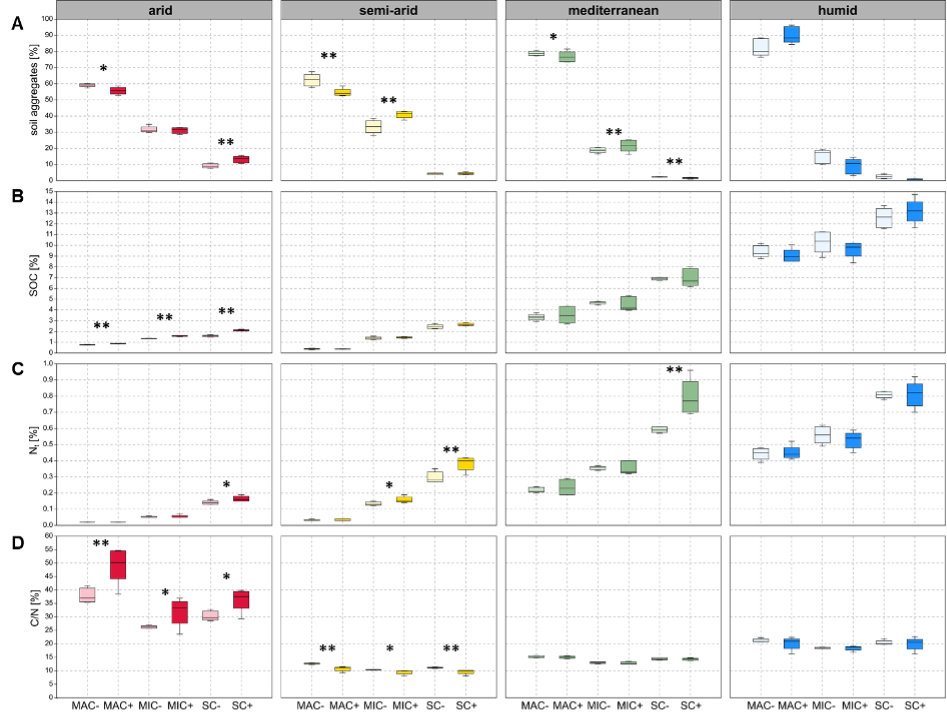
\includegraphics[width=1\textwidth]{img/M4-Figure_2.png}
	\caption{Soil properties in native soils (+) and sterilized soils (-) of different climates. 
    A) Aggregate size distribution. 
    B) SOC content, 
    C) TN content, and 
    D) C/N ratio per aggregate class. 
    MAC, macroaggregate fraction \SIrange{250}{2000}{\micro\metre}; 
    MIC, microaggregate fraction \SIrange{20}{250}{\micro\metre}; 
    SC, silt/clay fraction \SI{< 20}{\micro\metre}. 
    Significant differences between native and sterilized soils are indicated by asterisks (* \(p < 0.05\); ** \(p < 0.01\)).}
	\label{fig:M4-F2}
\end{figure}

Macroaggregates (MAC), microaggregates (MIC) and the silt/clay (SC) classes were differently distributed in arid, semi-arid, mediterranean and humid soils (Figure \ref{fig:M4-F2}a). Less developed soils from arid and semi-arid climate conditions were characterized by the lowest content of MAC ranging around \SIrange{60}{65}{\percent}. Semi-arid soils displayed a higher MIC content and a lower SC content compared to arid soils. More developed soils from the mediterranean and humid climates were characterized by the highest abundance of MAC with nearly \SI{80}{\percent} in mediterranean soils and more than \SI{90}{\percent} in humid soils. Accordingly, the proportion of MIC was low in mediterranean soils (\(\sim\)\SI{20}{\percent}) and lowest in humid soils (\SI{< 20}{\percent}). Moreover, SC was hardly present in mediterranean and humid soils (\(\sim\)\SI{2}{\percent}).

In native soils, including the indigenous microbial communities MAC contents decreased in arid, semi-arid and mediterranean soils, but increased in humid soils. 
MIC contents remained stable in arid soils, increased in semi-arid and mediterranean soils, but decreased in humid soils. 
The SC class slightly increased in arid soils, remained stable in semi-arid and mediterranean soils, and decreased in humid soils.

The SOC and TN (Figure \ref{fig:M4-F2}b-c) contents were lowest in the less developed soils and increased with soil development along the climate gradient, with the lowest SOC (\(\sim\)\SI{1}{\percent}) and TN values (\(\sim\)\SI{0.1}{\percent}) in arid soils and highest values in humid soils (\(\sim\)\SI{10}{\percent} and \(\sim\)\SI{0.5}{\percent}). In each soil, the SOC and TN contents were lowest within the MAC class and highest within the SC class. The C/N ratios (Figure \ref{fig:M4-F2}d) were highest in arid soils. Lowest values were observed in semi-arid soils with an increasing trend over mediterranean to humid soils. Within each soil, the highest C/N ratios can be observed within MAC, followed by SC and MIC.

The aggregate stability (MWD) was lowest in arid and semi-arid soils, increased in mediterranean soils and peaked in humid soils.

A principal component analysis (PCA) including soil aggregate size classes, aggregate stability (MWD), SOC, TOC and TN content as well as the C/N determined during repeated W-D cycles (Figure \ref{fig:M4-F3}a) revealed similar soil properties in native and sterilized soils from the same climatic condition. The separation of soils along the x-axis, explaining \SI{66.0}{\percent} of the variance, was in accordance with the climate gradient from arid to humid conditions. The difference between arid and semi-arid soils was mainly visible on the y-axis, explaining \SI{27.6}{\percent} of the variance. In addition, native and sterilized soils from arid conditions were separated along the y-axis.

\begin{figure}[H]
	\centering
	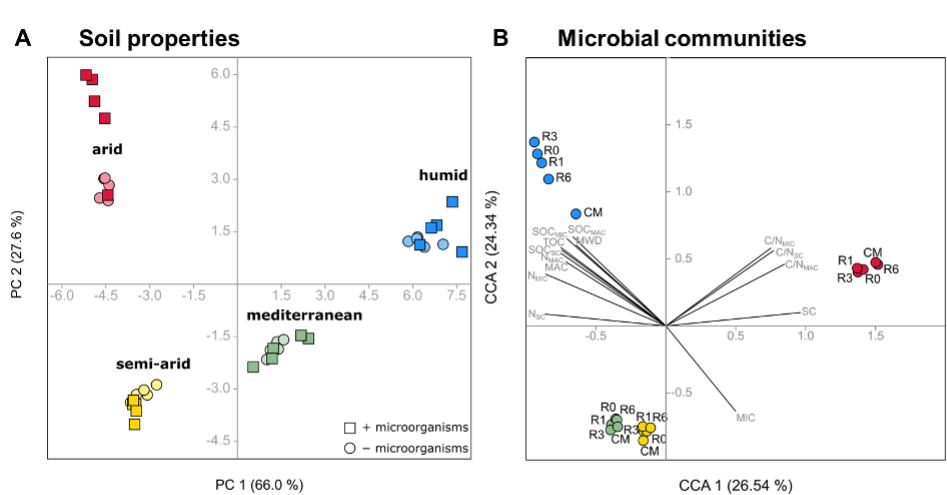
\includegraphics[width=1\textwidth]{img/M4-Figure_3.png}
	\caption{Soil properties and microbial community structure in soils of different climates. A) Principal Component Analysis of soil properties in native soils (squares) and sterilized soils (circles) including MWD, TOC, soil aggregates, SOC, TN and C/N per aggregate size class. B) Canonical correspondence analysis of the ASV composition including soil properties: MWD, aggregate class (MAC, MIC, SC) and the respective C/N ratio, SOC and TN content. R0-R6; number of W-D repetitions; CM, constant moisture. Colors represent different climatic conditions.}
	\label{fig:M4-F3}
\end{figure}

\subsection{Microbial influence on soil properties}

Differences between native and sterilized soils were further evaluated in separate PCA ordinations, showing significant differences between native soils and sterile controls not only in arid (\(p = 0.005\)), but also in semi-arid (\(p = 0.008\)) and mediterranean soils (\(p = 0.02\)) (Figure \ref{fig:M4-F4}). At these three sites, the native samples with microorganisms before W-D treatment (\(\square\)R0) were similar to all sterile controls (\(\circ\)R0--R6, CM) and were thus referred to as microbially not (yet) influenced. After at least 1 W-D cycle, microbial samples clustered apart from the sterile controls and were thus claimed to be microbially influenced. The difference between microbially influenced and not influenced samples appeared mainly along the x-axis of the plots, which explained the highest variance. In arid soils, the microbially influenced soils were characterized by higher C/N ratios in all aggregate classes (Figure \ref{fig:M4-F4}a). In semi-arid and mediterranean soils, soil aggregate sizes in microbially influenced soils were characterized by higher levels of MIC and C/N\textsubscript{SC}, and lower levels of MAC compared to the sterile controls (Figure \ref{fig:M4-F4}b-c). Microbially influenced humid soils were not significantly different from sterile soils. However, the majority of microbially influenced soils was characterized by higher MAC and MWD, while sterile soils had higher MIC contents (Figure \ref{fig:M4-F4}d).

\begin{figure}[H]
	\centering
	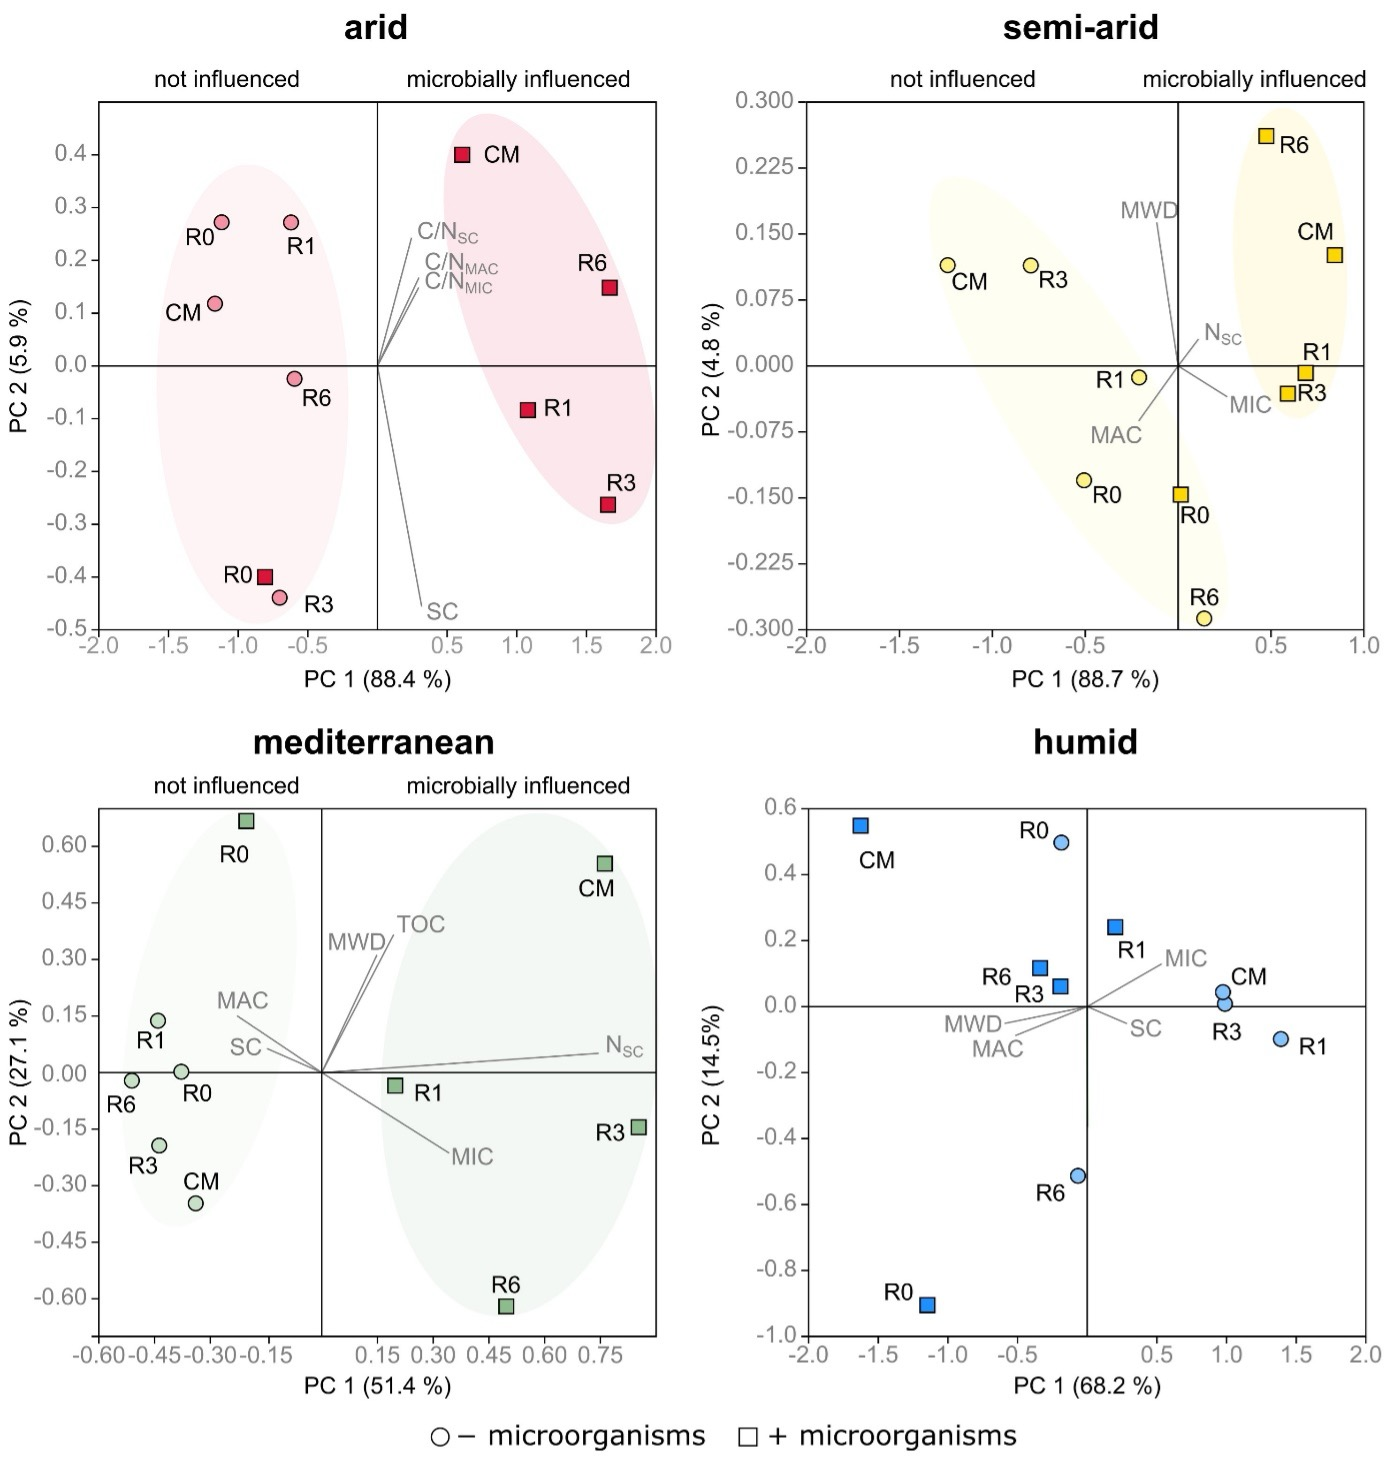
\includegraphics[width=1\textwidth]{img/M4-Figure_4.jpg}
	\caption{Principal Component Analyses of soil properties in native soils (squares) and sterilized soils (circles) including significant soil properties. A) arid, B) semi-arid, C) mediterranean and D) humid site. Microbial influence is indicated by sample separation along the x-axis.}
	\label{fig:M4-F4}
\end{figure}

\subsection{Microbial abundance}

Based on 16S and 28S rRNA gene copy numbers, bacteria were most abundant among all four climate conditions, followed by archaea and fungi (Figure \ref{fig:M4-F5}a). Only in humid soils, fungi were slightly more abundant than archaea and possessed highest abundances among soils. The lowest abundances of bacteria, archaea and fungi were observed in arid soils. Still, they increased over the course of the experiment with a peak after 3 cycles and maximum values under constant moisture. Semi-arid and mediterranean soils were characterized by highest abundances that remained relatively constant during the W-D cycles and constant moisture. In humid soils, bacterial and archaeal abundances were stable and fungal gene copies increased after 3 W-D cycles. However, all gene abundances of humid soils were lowest in soils exposed to constant moisture.

Linear (Pearson) and non-linear (Spearman) correlation analyses revealed that bacterial and archaeal abundances were positively correlated with each other. Both were inversely correlated with the C/N ratios in each soil class. On the contrary, the fungal abundance was positively correlated with MAC and MWD, while being inversely correlated with MIC and the S/C class. Furthermore, fungi were positively correlated with the SOC and TN contents in each aggregate class.

\begin{figure}[H]
	\centering
	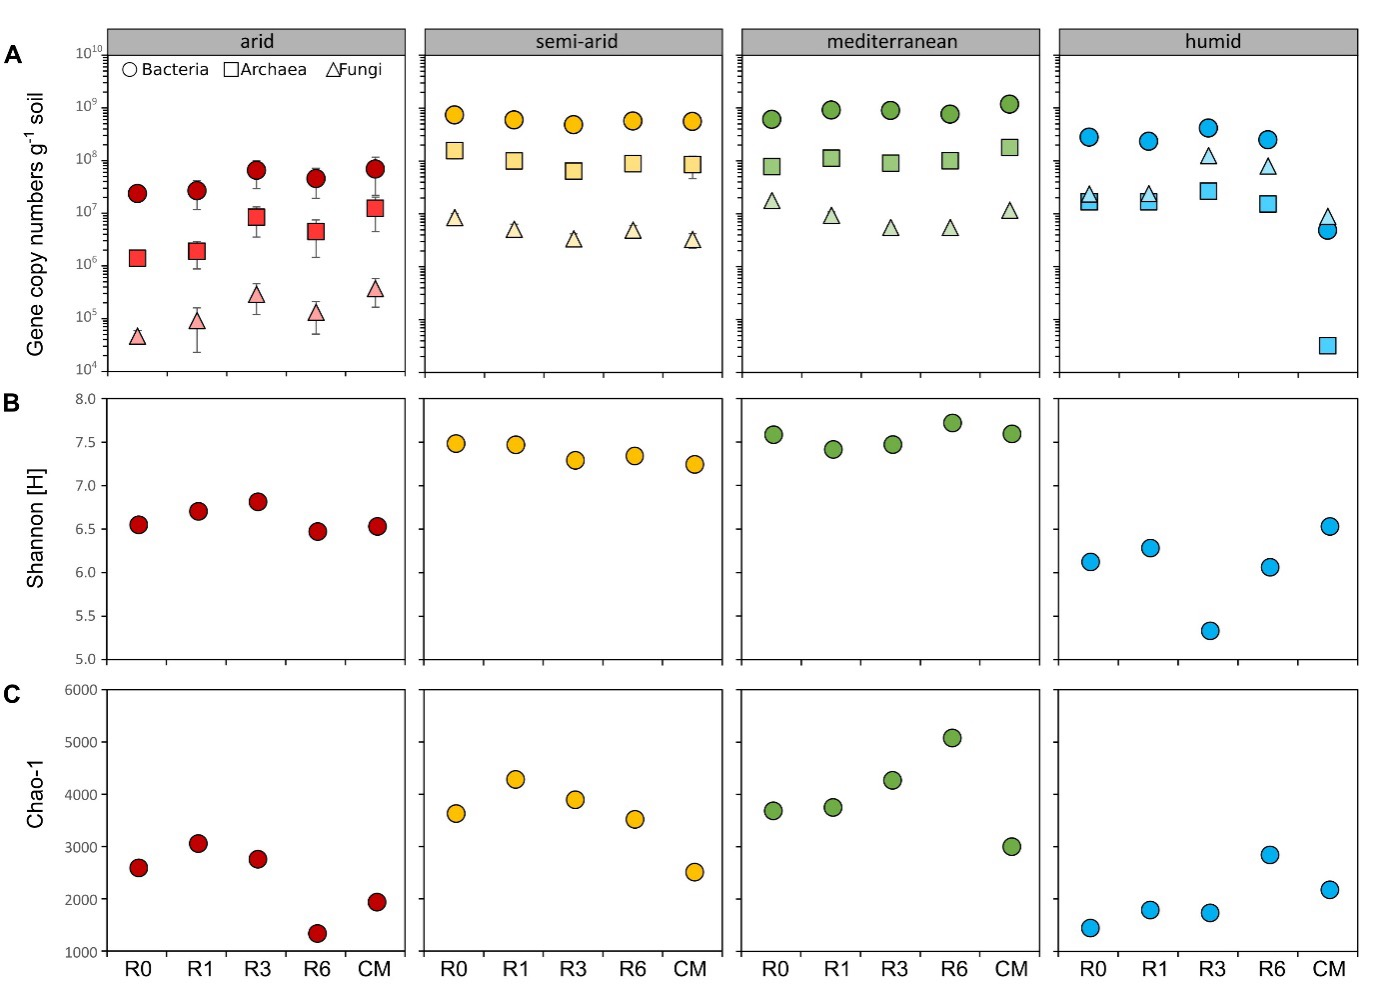
\includegraphics[width=1\textwidth]{img/M4-Figure_5.jpg}
	\caption{Prokaryotic and fungal abundance as well as prokaryotic diversity in soil material from different climates. A) 16S and 28S rRNA gene abundances of bacteria, archaea and fungi. Bacterial and archaeal diversity based on B) Shannon and C) Chao-1 diversity indices. R0 - R6, number of W-D repetitions; CM, constant moisture}
	\label{fig:M4-F5}
\end{figure}

\subsection{Bacterial and archaeal diversity}

Similar to their abundance, bacterial and archaeal diversity based on the alpha-diversity indices Chao-1 and Shannon (\(H\)) was highest in semi-arid soils from Santa Gracia (median \(H = 7.4\)) and in mediterranean soils of La Campana (\(H = 7.5\)) with maximum diversity indices in mediterranean soils (Figure \ref{fig:M4-F5}b). Although lowest microbial abundances were observed in arid soils, the bacterial and archaeal diversity was lowest in humid soils from Nahuelbuta (\(H = 6.0\)), followed by arid soils from Pan de Az{\'u}car (\(H = 6.6\)). In arid and semi-arid soils, the diversity according to Chao-1 increased after one W-D cycle and decreased afterwards. Contrary, mediterranean and humid soils were characterized by an increasing diversity during W-D cycles, but possessed a low diversity in the sample exposed to constant moisture. Like the bacterial and archaeal abundance, the number of taxa and the diversity were negatively correlated with the C/N ratios in all soil classes.

\subsection{Microbial community structure and composition}

Like the soil edaphic properties, the microbial communities clustered according to the climatic condition of each study site (Figure \ref{fig:M4-F3}b). In semi-arid and mediterranean soils, microbial communities did not significantly change during the treatment. Both communities were similar and clustered apart from those of arid and humid soils along CCA 2. While microbial communities of the semi-arid and mediterranean soils were similar (along CCA 1), soil parameters of the respective sites differed significantly (along PC 1). In contrast, microbial communities in humid soils displayed an increasing variance along the y-axis (explaining \SI{24.3}{\percent} of the variance) with increasing number of W-D cycles and under constant moisture. Similarly, the microbial communities of R6 and CM in arid soils varied from R0--R3 along the x-axis (explaining \SI{26.5}{\percent}).

The microbial community composition was assessed by MiSeq amplicon sequencing. After quality check and filtering (including removing reads of the negative control) the dataset comprised 1.2 million reads across \(\sim\)\num{11000} amplicon sequencing variants (ASVs). From this \(\sim\)\SI{98.1}{\percent} of the reads were assigned to bacteria and \SI{1.9}{\percent} to archaea. After taxonomic classification, 828 putative genera (807 for bacteria, 21 for archaea) were obtained. Based on phylogenetic classification, ASVs could be assigned to the ten dominant prokaryotic phyla Proteobacteria (\SI{24.8}{\percent} of total ASVs), Actinobacteriota (\SI{22.9}{\percent}), Acidobacteriota (\SI{11.9}{\percent}), Chloroflexi (\SI{8.7}{\percent}), Planctomycetota (\SI{8.5}{\percent}), Bacteroidota (\SI{5.1}{\percent}), Gemmatimonadota (\SI{4.8}{\percent}), Verrucomicrobiota (\SI{3.6}{\percent}), Firmicutes (\SI{2.3}{\percent}) and Crenarchaeota (\SI{1.8}{\percent}).

The bacterial communities of all four sites comprised 63 families and 18 unknown orders (Figure \ref{fig:M4-F6}). 
Of these families, 32 possessed almost or more than \SI{2}{\percent} mean relative abundance per site. 
Some were abundant (\SI{> 2}{\percent}) only at one site, while others were found in soils from several climatic conditions. 
Euzebyaceae, Pseudonocardiaceae, Caldilineaceae, AKYG1722 and JG30-KF-CM45 (Thermomicrobiales), Trueperaceae, Longimicrobiaceae, Pirellulaceae and unclassified Rhizobiales were abundant exclusively in arid soils from Pan de Az{\'u}car. 
Nitrososphaeraceae, Geodermatophilaceae, Micromonosporaceae and Beijerinckiaceae were abundant in the semi-arid soils of Santa Gracia. 
Vicinamibacteraceae and unclassified Vicinamibacterales were found to be abundant in mediterranean soils of La Campana. 
In contrast, Subgroup 1 of Acidobacteriales, Acidothermaceae, Ktedonobacteraceae, Gemmataceae and unclassified Elsterales were abundant only in the humid soils of Nahuelbuta.

\begin{figure}[H]
	\centering
	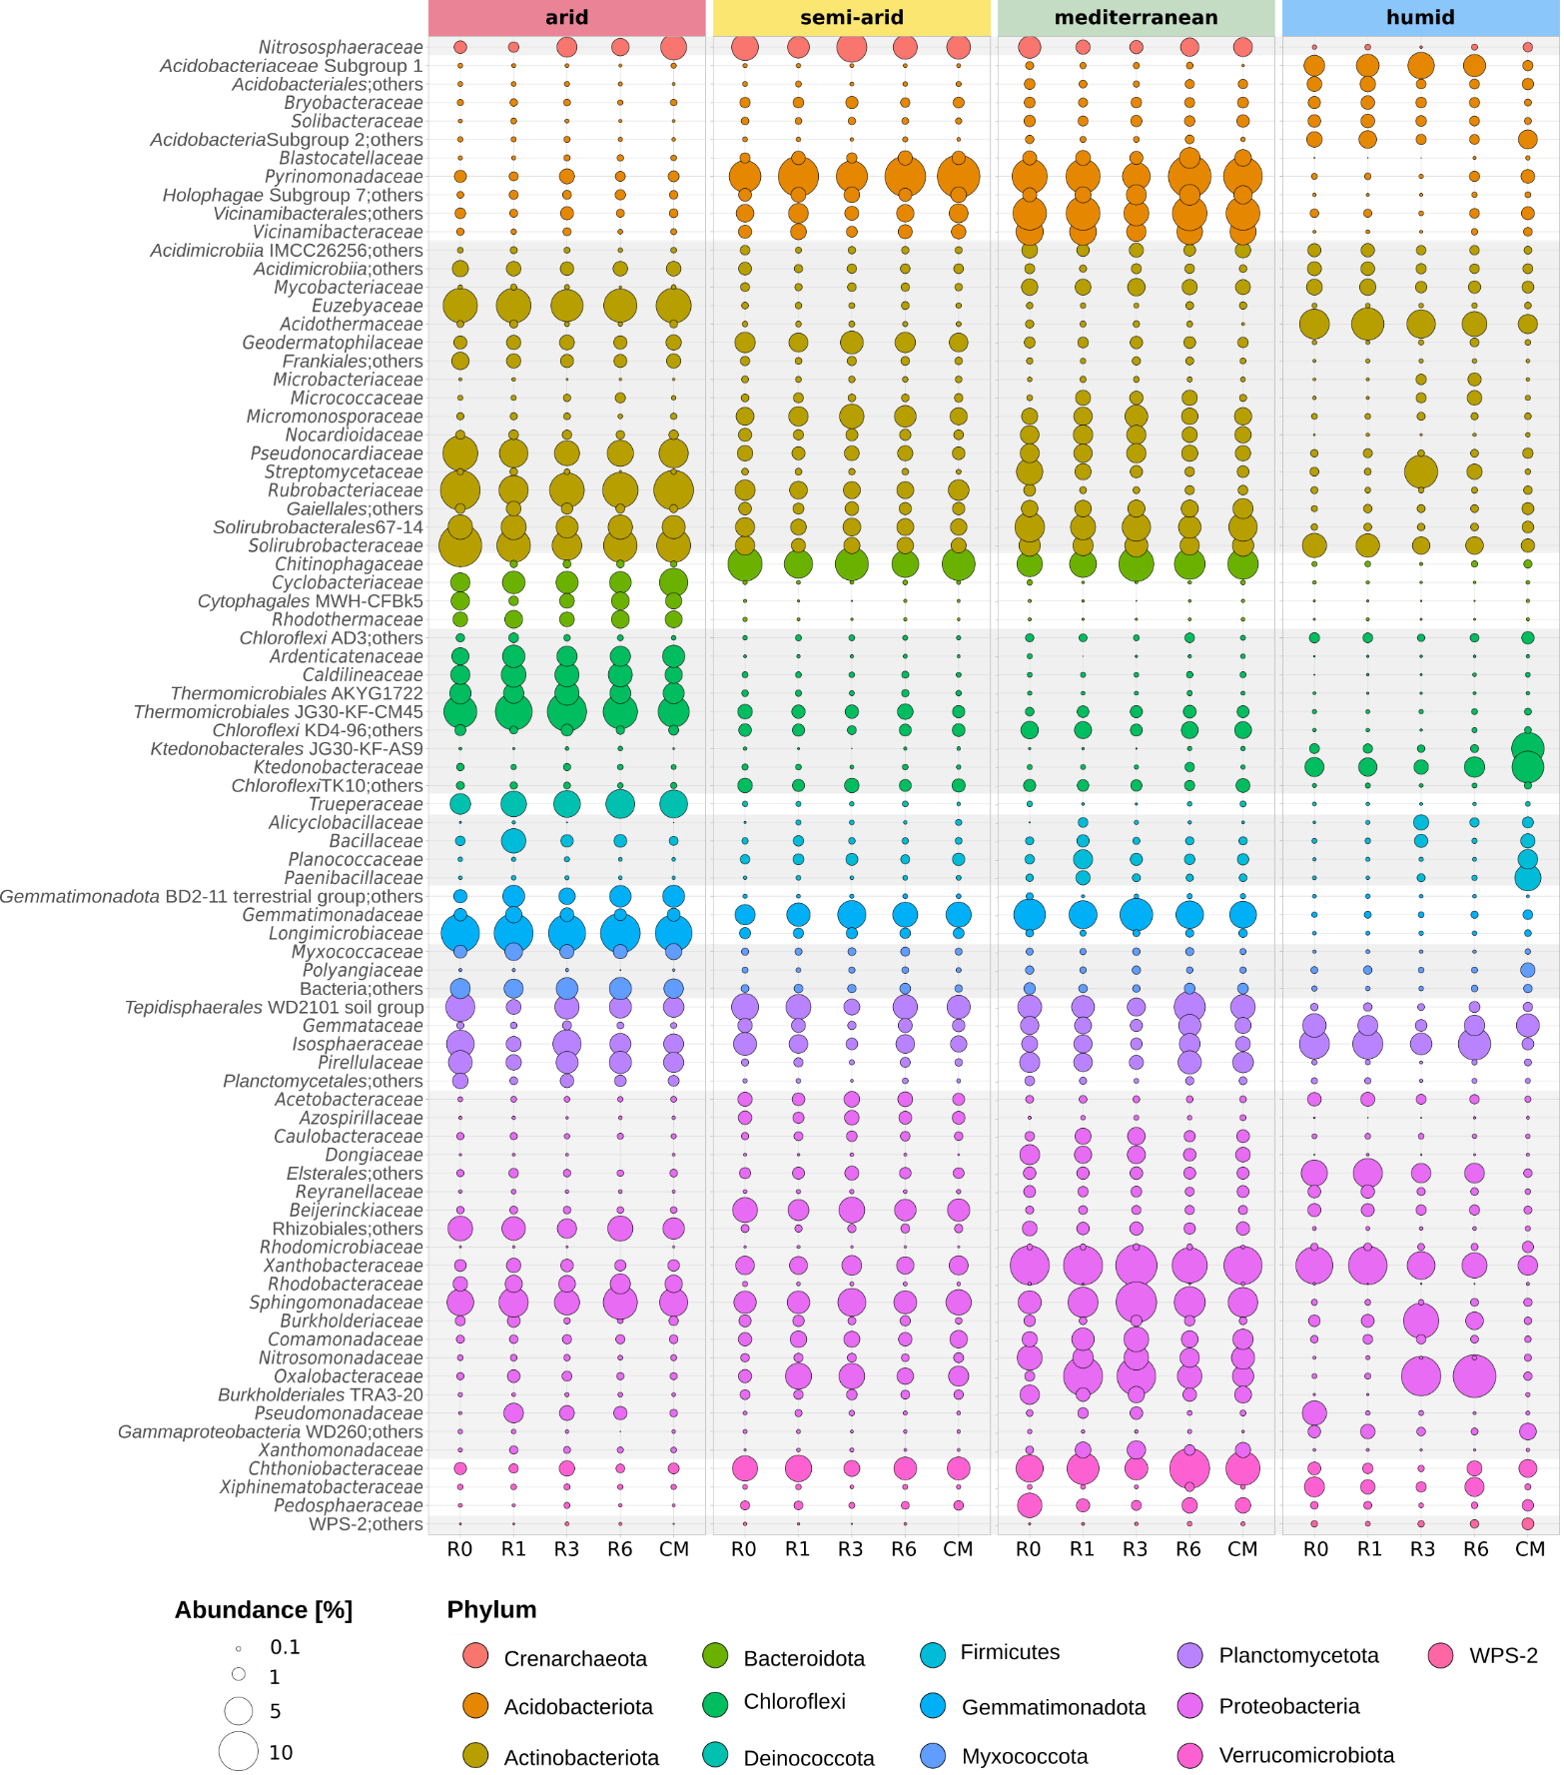
\includegraphics[width=1\textwidth]{img/M4-Figure_6.png}
	\caption{Relative abundance of prokaryotic families in soil material from different climates and after different soil treatments. R0-R6; number of W-D repetitions; CM, constant moisture. Each bubble represents the mean relative abundance of technical replicates.}
	\label{fig:M4-F6}
\end{figure}

\subsection{Predicted microbial functions}

Almost \num{11000} ASVs were assigned to 45 ecologically relevant functions using FAPROTAX, with 24 functions of significant abundance (cumulative abundance \SI{> 1}{\percent} across sites). 
In general, those predicted functions were related to organic matter degradation (chemoheterotrophy, fermentation, cellulolysis) phototrophy (anoxygenic photoautotrophy, photoautotrophy, photoheterotrophy and phototrophy), the nitrogen cycle (denitrification, nitrate denitrification, nitrate reduction, nitrate respiration, nitrification, nitrite denitrification, nitrite respiration, nitrogen fixation, nitrogen respiration, nitrous oxide denitrification) and degradation processes such as aromatic compound and hydrocarbon degradation as well as ureolysis. 
The most abundant predicted functions were related to chemoheterotrophy and aerobic chemoheterotrophy. In arid soils, additionally nitrate reduction (\SIrange{4}{7.5}{\percent}), nitrification and aerobic ammonia oxidation (\SIrange{0.5}{3.1}{\percent}) were enhanced. Some predicted functions decreased after the first W-D cycle (aerobic heterotrophy, chemoheterotrophy, manganese oxidation, nitrate reduction, nitrate respiration and nitrogen respiration), while others were enhanced after 1 and/or 3 W-D cycles (phototrophy, aromatic compound degradation, cellulolysis, ureolysis and many nitrogen cycle-related functions such as denitrification, hydrocarbon degradation, denitrification, nitrite respiration, nitrogen fixation, nitrous oxide denitrification). In semi-arid soils, again nitrate reduction (\SIrange{2.4}{3.5}{\percent}), nitrification (\SIrange{3.1}{4.6}{\percent}) and aerobic ammonia oxidation (\SIrange{3.0}{5.8}{\percent}) were enhanced following heterotrophy. Despite low abundances, many predicted functions were increased after 3 W-D cycles and most of them also in constantly moist soils. Similar observations were made in mediterranean soils. Humid soils were characterized by an enhanced abundance of ureolysis with an increasing trend, and cellulolysis as well as nitrogen fixation, with a decreasing trend during W-D treatment. The decreasing abundance was observed also for several other functions, while aerobic ammonia oxidation, fermentation, nitrification, phototrophy and photoheterotrophy were most abundant under constant moisture conditions.

\subsection{Correlation of microbial taxa with soil properties}

Correlation analyses of prokaryotic families and soil parameters revealed significant linear correlations (Pearson correlation; \(p < 0.05\)) of the edaphic parameters with 29 bacterial families in arid soils, with 26 in semi-arid soils, with 24 in mediterranean soils and with 43 families in humid soils. In arid soils, significant correlations of microbial families such as Holophagae subgroup 7, Acidimicrobiia, Frankiales, Pseudonocardiaceae, Solirubrobacteraceae, Trueperaceae, Caulobacteraceae, Rhodobacteraceae and Comamonadaceae were mainly observed with the C/N ratio. In semi-arid soils, significant correlations were primarily observed between the changing MAC and MIC content and families like Acidobacteria subgroup 2, Holophagae subgroup 7, Euzebyaceae, Caldilineaceae, Thermomicrobiales JG30-KF-CM45, Trueperaceae, Alicyclobacillaceae, Planococcaceae, Reyranellaceae, Comamonadaceae, Nitrosomonadaceae and WPS-2. In mediterranean soils, many correlations of bacterial families were observed with the aggregates, SOC\textsubscript{SC} and TN\textsubscript{MIC}. Thermomicrobiales JG30-KF-CM45, Dongiaceae, Rhizobiales and Burkholderiales TRA3-20 were related with the aggregate content, while Acidimicrobiia IMCC26256, Micrococcaceae, Cyclobacteriaceae, Ardenticatenaceae, Reyranellaceae, Rhizobiales and Burkholderiales were related with the SOC and TN content. In humid soils, numerous bacterial families were positively correlated with the duration of moisture application i.e. the number of W-D cycles or the duration of constant moisture in days. Families related with the soil moisture were affiliated with Nitrososphaeraceae (Crenarchaeota), Blastocatellaceae, Pyrinomonadaceae, Vicinamibacteraceae, Euzebyaceae (Acidobacteriota), Nocardioidaceae, Rubrobacteriaceae, Gaiellales, Solirubrobacterales (Actinobacteriota), Cytophagales (Bacteroidota), Ardenticatenaceae, Caldilineaceae, Thermomicrobiales AKYG1722 and JG30-KF-CM45, KD4-96, Ktedonobacterales JG30-KF-AS9, Ktedonobacteraceae, Chloroflexi TK10 (Chloroflexi), Trueperaceae (Deinococcota), Planococcaceae, Paenibacillaceae (Firmicutes), Gemmatimonadota BD2-11 terrestrial group, Gemmatimonadaceae, Longimicrobiaceae (Gemmatimonadota), Myxococcaceae, Polyangiaceae (Myxococcota), Rhizobiales, Rhodomicrobiaceae, Nitrosomonadaceae, Oxalobacteraceae (Proteobacteria), Pedosphaeraceae (Verrucomicrobiota) and WPS-2.

\section{Discussion}

In this study, we explored the combined effect of abiotic (water) and biotic (microbial activity) factors on the formation and persistence of soil aggregates. Studying sterilized in parallel to native soil materials allowed us to determine the biotic, i.e. microbial contributions to the formation and stabilization of soil aggregates in comparison to abiotic processes.

The four study sites along the Chilean Coastal Cordillera comprised soils ranging from poorly developed soils such as Regosol in the arid north to more developed soils such as Cambisols (semi-arid and mediterranean study sites) and to Umbrisols in the humid south. The soils were characterized by increasing clay, soil organic matter, soil moisture contents and soil acidity from north to south \citep{Bernhard2018} (\ref{fig:M4-F2}) and, thus provide different initial conditions for studying the microbial impact on soil aggregation and stabilization.

The level of soil development was not only indicated by the distribution of soil aggregate size classes but also by organic C and N contents of the particular soil aggregate classes. Overall, lowest SOC and TN contents were observed in the MAC fraction. They were higher in MIC and highest in the SC fraction. Clay and silt are known to build strong relations with stable humic substances \citep{Bouajila2021} and protect them against decomposition by microbial activity. Across sites, arid soils were characterized by maximum C/N ratios, typical for soil systems with a high amount of recalcitrant organic matter that is decomposed very slowly. Although, MIC are characterized by having increased amounts of biochemically recalcitrant C (i.e. compounds with a higher C/N ratio) \citep{Elliott1986, Kravchenko2015}, we observed highest C/N ratios in the MAC fractions of all four soil types. In accordance with previous work \citep{Kuramae2012}, the C/N ratio appeared to be a strong driver of the microbial community composition (Figure \ref{fig:M4-F3}b) as well as of abundance and diversity.

\subsection{Microbial influence on soil aggregation}

Wetting and drying of soil material from the arid site led to significant differences in the soil edaphic properties between sterile and microbially influenced soil materials (\ref{fig:M4-F4}). The microbially influenced soil material was characterized by increased C/N ratios in all soil aggregate classes compared to sterile soil material, with the highest C/N ratios in MAC (\ref{fig:M4-F2} \& \ref{fig:M4-F4}). Increased C/N ratios indicate accelerated microbial activity and labile soil organic matter (SOM) turnover in all aggregate classes. This is corroborated by an increase in microbial abundance with increasing number of W-D cycles. In addition, W-D of native soil material was accompanied by a loss of MAC, a slight loss of SOC\textsubscript{MAC} and N\textsubscript{MAC} but a gain of MIC, a slight gain of SOC\textsubscript{MIC} and SC compared to sterile soil material. The microbial decomposition of aggregate-associated OM might lead to aggregate disintegration and thus initiate aggregate turnover \citep{Six2000}. On the other hand, disruption of MAC may have enhanced OM mineralization \citep{Goebel2009, Mueller2012}. Despite an increasing abundance of fungi, which usually contribute to the formation and stabilization of MAC due to mycorrhizal mycelia \citep{Chotte2005, Lehmann2017}, W-D of native arid soil material promoted the breakdown of MAC, liberating MIC and SC. Our results support the findings that MAC are less stable than MIC \citep{Six2004, Tisdall1982} and that W-D decrease MAC stability \citep{Lehrsch1991, Mulla1992, Zhang2022}. The potentially decreasing MAC stability in addition to the loss of MAC led to a slight decrease of the aggregate stability (MWD). As MAC are assumed to contain more labile SOM than MIC \citep{Elliott1986}, their disintegration may have fueled the release of locked labile organic matter, raising microbial respiration from the decomposition \citep{Najera2020} and resulting in the increased C/N ratio. W-D processes are a significant driver for reorienting aggregate building units and developing a three-dimensional soil structure \citep{Chenu2011}. In our soil manipulation experiment, the decreasing aggregate stability may be a result of the absence of plant roots, which usually promote MAC formation and thus act as drivers of soil aggregate stability and organic carbon accumulation \citep{Blankinship2016, Erktan2016, Rodriguez2024}.

In soil materials from the semi-arid and mediterranean sites, highest bacterial and archaeal abundances as well as diversity were inversely related with lowest C/N values across sites. Soils with low C/N values are usually characterized by having higher concentrations of labile organic matter that is more easily decomposed \citep{Kuramae2012} and can provide a favorable environment for microorganisms to thrive. Despite differences in soil aggregate distributions as well as SOC and TN contents (\ref{fig:M4-F2} \& Figure \ref{fig:M4-F3}a), both, semi-arid and mediterranean soils were classified as Cambisols \citep{Bernhard2018} and we observed a similar microbial impact on the soil properties. MIC and TN contents were higher in microbially influenced soil materials compared to the sterile soil material (\ref{fig:M4-F4}). Particularly in semi-arid soil material, the high MIC content was related to the microbial diversity and the high microbial abundance, corroborating that MIC formation and stabilization is mainly caused by microbial-derived binding agents \citep{Six2004}. 
The gain of MIC and the associated loss of MAC compared to sterile soil material was more pronounced in semi-arid than in mediterranean soil material, resulting in a slight but not significant change of aggregate stability (\(p = 0.08\) in semi-arid, \(p = 0.06\) in mediterranean soil). While the aggregate stability slightly decreased in semi-arid soils, it slightly increased in mediterranean soil material. In the latter, the gain of MIC could be partially the result of MIC formation from SC, as its content decreased. In addition, the mediterranean soil material was characterized by a generally higher MAC content and a slightly higher fungal abundance, which potentially stabilized MAC and supported MIC formation, leading to the elevated aggregate stability \citep{Chotte2005}. Soils exposed to alternating moisture conditions, like the mediterranean soils which originate from a climatically unstable ecosystem \citep{Rodriguez2022}, were suggested to have a stronger resilience against temporary variations in these conditions than soils that are rarely water saturated \citep{Totsche2018}. The elevated sand content in semi-arid and mediterranean soil material from Santa Gracia and La Campana \citep{Bernhard2018} may have restricted the impact of bacteria and archaea on the soil aggregates, as in coarser textured sandy soils aggregation is less related to microbial biomass and products \citep{Degens1996}. However, the hyphal network of fungi, which were found to be more abundant in semi-arid and mediterranean soil material, is able to cross-link the abundant sand particles to form stable aggregates \citep{Six2004}. Respectively, they were significantly positive correlated with aggregate stability and SOC, TN and C/N ratio.

Along with the loss of MAC in microbially influenced semi-arid soil material, the SOC and TN content in the MIC and the SC fraction increased compared to sterile soil material (Figure \ref{fig:M4-F2}) indicating a release of SOC and TN during the disintegration of MAC, which are usually enriched in labile carbon and nitrogen \citep{Marx2005}.

In mediterranean soil material, the microbial influence was characterized by a loss of SOC and TN with the number of W-D cycles in all aggregate size fractions, indicating microbial activity. This was accompanied with a weak rise of the prokaryotic abundance and diversity. Only the TN\textsubscript{SC}, which correlated with the bacterial abundance, increased significantly.

The humid soil in Nahuelbuta represents an old, developed, and stable landscape \citep{Mucina2011}. This soil material was characterized by maximum MAC, SOC and TN contents as well as the highest aggregate stability (\ref{fig:M4-F2}). Remarkably, aggregate stability was significantly higher in microbially influenced soil material (\(p = 0.02\)). This was accompanied by maximum fungal gene abundances with an increasing trend during W-D, and a significant correlation between fungal abundance and MWD. Our observations coincide with previous studies demonstrating that fungal biomass correlated with aggregate stability \citep{Cosentino2006}, fungi occur more abundantly in association with MAC \citep{Kihara2012} and that soil mycorrhizal fungi play a key role in MAC formation and stabilization \citep{Chotte2005}. MAC are formed due to fungal hyphae, which physically enmesh soil particles and MIC \citep{Davinic2012}. Despite the generally higher MAC and lower MIC contents (\ref{fig:M4-F2}) and, thus, higher aggregate stability, soil parameters in microbially influenced soil material including aggregate classes, C, TN and C/N contents as well as MWD were not significantly different from sterile soil material (\ref{fig:M4-F4}). However, under constant moisture conditions we observed a significant reduction of the abundance of bacteria, archaea and fungi (Figure \ref{fig:M4-F5}a) with a concomitant increase in MAC and a loss of MIC. Besides the fungal abundance, aggregate stability can also be linked with the SOC content \citep{AlKaisi2014}. Particularly under wetter conditions in bare soil, organic matter can strongly impact soil aggregation, exceeding the influence of microorganisms \citep{RiverasMunoz2022}. The gain of MAC\textsubscript{SOC} observed under constant moisture conditions may be attributed to deceased microbial cells resulting from the drastic loss of microbial abundance. This could have contributed to the formation of MAC in microbially influenced soil material.

\subsection{Microbial response to W-D cycling and key taxa of soil alteration}

The microbial response to W-D cycles and its effect on soil aggregate dynamics was analyzed by means of changing gene copy abundances, diversity and a changing microbial community composition and structure in relation to soil edaphic properties.

In arid soil material, the increasing microbial abundance (including fungi) and a changing microbial diversity (Figure \ref{fig:M4-F5}b-c) are likely the response to the availability of water. The so called 'Birch effect' promotes the breakdown of aggregates, mineralization of dead microbial cells and osmolytes, and a subsequent release of nutrients such as C \citep{Jarvis2007}. Particularly in arid and semi-arid soils, this effect combined with MAC breakdown enhances bacterial reproduction and growth by releasing organic compounds \citep{Armstrong2016, Seuss2022}. This effect may have resulted in the observed peak of microbial abundance and diversity after 1 or 3 W-D cycles (Figure \ref{fig:M4-F5}b-c), accompanied by an increase in predicted functions. Following 6 W-D cycles the abundance of the majority of predicted functions decreased along with the microbial abundance and diversity (Figure \ref{fig:M4-F5}), while the community composition on ASV level slightly changed (Figure \ref{fig:M4-F3}b). W-D cycles can create dynamic shifts in microbial communities. During the wet phase, certain microbial groups, may benefit from the increased water availability, increasing the abundance and diversity of the community. Continuous W-D cycles may select for microbial taxa tolerant to desiccation stress \citep{Evans2012}, resulting in the observed loss of diversity and reconstitution of the predicted microbial functions. Our observations are in line with previous studies demonstrating that sudden climate shifts can act as stressors that promote a reduction of diversity \citep{Clavel2011}, particularly when water is rapidly and abundantly applied to hyper-arid soil \citep{AzuaBustos2018} and frequent W-D stress selects for tolerant microbial taxa \citep{Seuss2022}. Due to fewer available metabolic pathways, the loss of diversity could negatively affect the soil formation and stabilization \citep{Bestion2020, Shen2023}.

The low diversity in soil material of the arid study site, results from a high degree of bacterial specialization, which is attributed to an evolutionary response to a stable environment \citep{Rodriguez2022}. Despite the changing abundance, diversity and potential functions, the family-level microbial community composition was altered slightly but not significantly during the manipulation experiment (Figure \ref{fig:M4-F6}). Community composition changes can occur quickly within a single W-D cycle \citep{Evans2012} and, thus, may not be detectable after a completed W-D cycle. In addition, drivers of specific microbial functions can change without changing the microbial community itself.

Along with the prokaryotic abundance and diversity, we observed significant correlations of single bacterial families with soil properties such as C/N and MIC content. The elevated C/N ratios in microbially influenced soil materials were inversely correlated with the abundance of Acidimicrobiia, Frankiales, Pseudonocardiaceae (\SI{3.9}{\percent}) and Solirubrobacteraceae (\SI{5.7}{\percent}) (both Actinobacteriota) as well as Caulobacteraceae (Alphaproteobacteria), some of them being exclusively abundant in arid soil material. Other families such as Trueperaceae (\SI{3.2}{\percent}, Deinococcota), Rhodobacteraceae (\SI{1.4}{\percent}, Alphaproteobacteria), Comamonadaceae (Gammaproteobacteria) or Holophagae subgroup 7 (Acidobacteriota) were positively correlated to the increased C/N ratios, and thus negatively with the decreased TN content, indicating their participation in a potentially accelerated microbial turnover of labile soil organic matter and increase of the microbial abundance. These families were shown to be related to the soil nitrogen content. Trueperaceae are typical representatives of bare soils and early biocrust stages in drylands \citep{Albuquerque2005, Maier2018} as can be found in the biocrust-dominated desert of Pan de Az{\'u}car \citep{Bernhard2018}, and are often related to nitrogen removal \citep{GonzalezBlanco2020}. Also Rhodobacteraceae was related to nitrogen removal \citep{Jia2020}, and its abundance seemed to be induced by an increasing C/N ratio \citep{Guo2020}. In contrast, families such as Pseudonocardiaceae and Solirubrobacteraceae, known for the degradation of soil organic carbon (such as complex polysaccharides, cellulose, hemicellulose, chitin and xylan) \citep{Broadbent2022, Yeager2017} were negatively correlated with the increased C/N ratio, thus, decreased in their relative abundance. Hence, an increase of the C/N ratio was potentially caused by N removal due to an increased activity of corresponding bacterial groups. Accordingly, predicted functions such as nitrogen fixation and ureolysis, both resulting in the formation of ammonium, were stimulated. This was followed by an induction of aerobic ammonia oxidation, nitrification as well as nitrate reduction, potentially resulting in the release of gases that can escape into the atmosphere. At the same time, the abundance of chemoheterotrophic processes, that can reduce the soil carbon content, was reduced.

In addition, W-D of native soil material promoted a loss of MAC and a gain of MIC and SC, potentially caused by the disintegration of MAC and/or by binding small MIC through microbial-derived EPS \citep{Six2004, Totsche2018}. Sphingomonadaceae (Alphaproteobacteriota), keystone taxa in MIC and MAC \citep{Feng2022}, significantly correlated with the increased MIC content. \textit{Sphingomonas}, the most abundant genus within the Sphingomonadaceae, has been associated to MIC formation through the excretion of EPS \citep{Pankratov2007, Vuko2020}, while the family has been related to the EPS-saccharide content in soil \citep{Bettermann2021}. Furthermore, Chitinophagaceae (Bacteriodota), which was positively correlated to the SC content, has been described as keystone taxa in SC \citep{Feng2022}. Likewise, \textit{Holophaga}, which was found to be mainly present in smaller-size fractions \citep{Sessitsch2001}, potentially explains the correlation of Holophagae subgroup 7 with MIC and C/N\textsubscript{MIC}.

Contrary to the arid soil material, microbial abundance as a measure of activity was not as strongly stimulated but remained relatively stable in semi-arid and mediterranean soil material during the manipulation experiment (Figure \ref{fig:M4-F5}a). Similar to the abundance, the prokaryotic diversity and community composition (Figure \ref{fig:M4-F3}b, Figure \ref{fig:M4-F6}) of both soil types were comparable. A main explanation could be the similar soil acidity \citep{Bernhard2018}, which is controlled by the water balance as a result of the climate conditions \citep{Slessarev2016}. In addition, W-D of both soil types caused no significant changes of the community composition (\(p = 0.8\) in semi-arid, \(p = 1\) in mediterranean soil material). Despite the consistent community composition in both soil types, W-D resulted in a microbial response that had similar effects on the soil parameters (enhanced MIC and TN\textsubscript{SC} contents, but a loss of MAC), but different effects on aggregate stability.

Similar to the arid soil material, the diversity in the semi-arid soil material slightly decreased after an initial increase. Semi-arid soils of Santa Gracia usually experience one annual moisture pulse in the winter season, suggesting that sudden and repetitive shifts of the soil moisture could have acted as a stressor and promoted the reduction of diversity \citep{Clavel2011}. A selection of more tolerant microbial taxa by frequent W-D stress and the resulting smaller number of available metabolic pathways could have negatively affected the soil formation and stabilization \citep{Bestion2020, Shen2023} as observed by the loss of MAC and MWD. The loss of diversity, however, was less pronounced than in arid soil material. In contrast to the arid soils of Pan de Az{\'u}car, the semi-arid soils from Santa Gracia represent a rather heterogeneous and disturbed ecosystem dominated by bacterial generalists \citep{Rodriguez2022}, benefiting from their metabolic flexibility to thrive in dynamic environments \citep{Bai2021, ChenLeung2021, Hawkes2020}. Similarly, the mediterranean soils from La Campana originate from a topographically and climatically unstable ecosystem \citep{Rodriguez2022} that promotes a low number of bacterial specialists and explains the high diversity observed for both, semi-arid and mediterranean soil materials. At least during the winter season, soils in La Campana are subjected to repetitive rainfall events and periodical changes of the soil water content, resembling the conditions of this manipulation experiment \citep{Uebernickel2020}. Since soil material was sampled before the wet season (in March--April), W-D potentially induced a change in the prokaryotic community from drought tolerant taxa to W-D tolerant taxa, resulting in an increase in diversity and a slight increase in abundance. Although changes in semi-arid and mediterranean soil materials were insignificant, we observed an increasing relative abundance of several bacterial families with a peak after 3 W-D cycles (Figure \ref{fig:M4-F6}), accompanied by an abundance peak of nearly all predicted metabolic functions.

As in sandy soils, where aggregation is suggested to be weakly related to microbial biomass and products \citep{Degens1996}, we observed only a few correlations of microbial taxa with the soil aggregate distribution. In both soil materials, different bacterial families of lower relative abundance were significantly related to the changed MIC and TN\textsubscript{SC} content in microbially influenced soil material. In the semi-arid soil material, we observed positive correlations of Holophagae Subgroup 7 (\SI{1.3}{\percent}), Alicyclobacillaceae, Planococcaceae, Reyranellaceae, Comamonadaceae (\SI{1.5}{\percent}) and Nitrosomonadaceae with the increasing MIC content. Also in arid soil material, Holophagae Subgroup 7 and Comamonadaceae were linked to changing soil properties. Here, we suggested that Comamonadaceae have been involved in an accelerated microbial turnover of labile soil organic matter and an increase of the microbial abundance. Assuming that the gain of MIC partially results from the breakdown of MAC and a subsequent release of labile OM, their correlation with the increasing MIC content in semi-arid soil material would corroborate this assumption. In addition to MIC, Holophagae Subgroup 7, Planococcaceae, Reyranellaceae and Oxalobacteraceae (\SI{2.8}{\percent}) were positively correlated with the increased N\textsubscript{SC} content. \textit{Massilia}, the most abundant genus of the Oxalobacteraceae, are able to produce extracellular proteases, which can depolymerize high molecular weight detrital organic N. The resulting N monomers can be taken up by microorganisms leading to the excretion of amino acids and excess ammonium, thereby increasing the soil N content \citep{Sieradzki2023}.

In mediterranean soil material, we observed fewer correlations with MIC. Only Thermomicrobiales JG30-KF-CM45 was positively correlated with the gain of MIC and negatively with the loss of MAC. Positive correlations with N\textsubscript{SC} were observed for Chitinophagaceae (\SI{3.6}{\percent}, Bacteriodota) and Sphingomonadaceae (\SI{3.9}{\percent}, Alphaproteobacteriota), two abundant families in mediterranean soil material. Chitinophagaceae, keystone taxa in SC \citep{Feng2022}, are known for their ability to degrade long-chain polymers like chitin \citep{Proenca2017}. Chitin degradation has the potential to release nitrogen-containing compounds into the soil, contributing to the pool of available nitrogen. In addition, Sphingomonadaceae, usually related to bigger-sized soil aggregates \citep{Feng2022, Yang2019}, can be one of the critical nitrogen cycling families in soil \citep{Wang2020}. Some species of \textit{Sphingomonas}, besides Ellin6055, the most abundant genus within Sphingomonadaceae, are capable of nitrogen fixation \citep{Asaf2020}. Consequently, the predicted functions of nitrogen fixation and ureolysis increased with W-D, potentially increasing the soil TN\textsubscript{SC} content to levels comparable to the humid soil material of Nahuelbuta (\ref{fig:M4-F2}).

Like diversity, the abundance of bacteria and archaea was lower in humid than in mediterranean and semi-arid soil material. Moister soil conditions reduce diversity through dispersion, connectivity, homogenization, and nutrient fluxes \citep{StovicekA2017}. Similar to the mediterranean soil material, the abundance and diversity increased with W-D cycles, with an abundance peak after 3 W-D cycles but decreased upon constant moisture. Soils in Nahuelbuta are exposed to repetitive rainfall events and periodical changes in the soil water content throughout the year \citep{Uebernickel2020}. Hence, the manipulation experiment resembled the original conditions regarding the moisture pulses. However, the soil in Nahuelbuta does not normally experience drought as in the dry phase of the manipulation experiment. W-D potentially stimulated parts of the microbial community, by raising the microbial abundance and diversity, and induced a change of the highly specialized prokaryotic community, emanating from a stable ecosystem \citep{Rodriguez2022} to more desiccation tolerant taxa. In contrast, constant moisture resulted in a drastic loss of the fungal and prokaryotic abundances. Excess soil moisture, as a result of a high clay content, lower permeability, drainage, and thus aeration, is known to decrease the number of fungi, as they are strictly aerobic \citep{Chotte2005}.

Similar to the abundance, the bacterial and archaeal community response in terms of changing relative abundances of single families was significant and particularly pronounced after 3 W-D cycles and under constant moisture conditions. W-D led to an increasing relative abundance of Actinobacteriota (Streptomycetaceae), Firmicutes (Alicyclobacillaceae, Bacillaceae) and Proteobacteria (Burkholderiaceae,Oxalobacteraceae), but a decrease of Acidobacteriota, Chloroflexi, Planctomycetota (Gemmataceae, Isosphaeraceae) and Verrucomicrobiota (Chtoniobacteraceae, Xiphinetmatobacteraceae) (Figure \ref{fig:M4-F6}). Actinobacteriota and Proteobacteriota are copiotrophic phyla \citep{Finn2021, Li2021}, i.e. they are fast growing under high nutrient availability leading to highly variable population sizes. In contrast, Acidobacteriota, Chloroflexi, Planctomycetota and Verrucomicrobiota follow an oligotrophic life-strategy. They are generally slow-growing phyla with more stable population sizes \citep{Barnard2013, DelgadoBaquerizo2017a}. There is, however, little agreement on whether Firmicutes have a copiotrophic or oligotrophic lifestyle \citep{Schostag2019}. In the context of rising bacterial abundances, their loss of relative abundance may have resulted from an increasing abundance of the fast growing copiotrophic phyla, while abundances of the oligotrophs remained stable. Following 6 W-D cycles the relative abundances usually recovered. However, relative abundances of Chloroflexi (Ktedonobacterales JG30-KF-AS9, Ktedonobacteraceae) and Firmicutes (Planococcaceae, Paenibacillaceae) remained high under constant moisture, but decreased in Actinobacteriota, Planctomycetota and Proteobacteria. Regarding the generally low microbial abundances in constantly moist soil material, the increased relative abundance of Chloroflexi and Firmicutes indicated moisture stress-tolerance and a stable life-strategy. Several members within the Firmicutes are capable of producing endospores, including \textit{Paenibacillus} \citep{Paredes2005, Schostag2019}. Despite the reduced relative abundance of above-mentioned phyla in constant moisture conditions, a number of archaeal and bacterial families, affiliated with all abundant phyla except Planctomycetota, were positively correlated with the duration of soil moisture exposure. They were also related to the increased MAC content, however, only a few significantly correlated.

Our study demonstrates that during wetting and drying, various predicted microbial functions associated with chemoheterotrophy, cellulolysis, nitrogen fixation, and ureolysis showed a decline. This decline was most pronounced under constant soil moisture conditions, presumably due to reduced aeration. The diminished functions of chemoheterotrophy and cellulolysis suggest a deceleration in organic matter and litter decomposition processes within the soil. This metabolic slowdown, particularly in constantly moist conditions, could have contributed to an accumulation of organic matter, fostering the formation of MAC. Furthermore, reducing nitrogen fixation activities implies a decrease in introducing new nitrogen into the soil ecosystem. This shortfall may curtail nitrogen availability, impacting microbial activities reliant on nitrogen. Notably, this reduction aligns with observed decreases in microbial abundance and soil nitrogen content resulting in an increased C/N ratio.

Under constant moisture conditions, less abundant predicted functions associated with aerobic ammonia oxidation, fermentation, nitrification, and phototrophy gained increased relevance. The stimulation of fermentation, suggests that the lack of oxygen, caused by water saturation, is at least partially responsible for this stimulation. Nitrification and ammonia oxidation lead to the conversion of ammonia to nitrate, which is more accessible to plants and affects the soil pH due to the release of H\textsuperscript{+}. These changes can influence organic matter accumulation, nutrient availability, and soil microbial processes, ultimately impacting soil health and ecosystem functioning. The stimulation of phototrophy and photoheterotrophy points to an initiation of biological soil crust (BSC) formation, where bacteria are contributors. BSC often act as pioneer communities developing after vegetation disturbances and affecting the stability of soil aggregates. In humid conditions, their role in aggregate stability is usually masked by higher vegetation and organic matter contents in the topsoil \citep{RiverasMunoz2022}. However, without plants, their potential impact becomes observable.

\section{Summary}

In arid native soils, we propose the Birch-effect stimulated microbial activity. The selective consumption of labile organic matter by microbes from MAC diminished the quality of organic matter and caused the breakdown of larger soil aggregates. Conversely, neither W-D nor constant moisture notably stimulated microbial activity in semi-arid soils. However, the microbial decomposition of organic matter from MAC might have resulted in the accumulation of SOC and TN in the MIC fraction through microbial binding agents, thereby fostering MIC formation and stabilization, ultimately decreasing aggregate stability. In mediterranean native soils, microbial activity was stimulated and likely facilitated the de novo assembly of MIC from components of the SC fraction. Despite reductions in the MAC content due to W-D and constant moisture, the higher fungal abundance potentially stabilized the remaining MAC. It supported MIC formation, thus augmenting soil aggregate stability alongside microbial-mediated MIC formation. Humid soils exhibited a distinctive response to moisture manipulation. A substantial fungal presence likely played a pivotal role in significantly enhancing aggregate stability. Furthermore, prokaryotic activity was stimulated by W-D. Conversely, microbial abundance experienced a substantial decline under constant moisture due to moisture stress, yet there was a noteworthy increase in aggregate stability. We suggest that particularly under moister soil conditions, the increased carbon content, resulting from deceased microbial cells, strongly impacts soil aggregation, facilitating MAC formation and elevating aggregate stability.

\section{Conclusions}

The composition and attributes of soil aggregates' building components and microbial communities, exhibit variation influenced by pedogenesis and prevailing climatic conditions. These variances contribute to differences in the mechanisms responsible for forming and stabilizing soil aggregates and dictate how microbial populations respond to changes in soil moisture levels. Without plant roots as binding agents, microbially influenced soils possessing lower to moderate organic matter content and initial soil water content displayed reduced macroaggregate abundance and soil aggregate stability following W-D cycles. Higher initial soil water content enhanced the resilience of aggregates in microbially influenced soils to disruptive forces. Our findings demonstrate the influence of microorganisms in soil formation, highlighting the role of historical soil conditions in shaping responses to environmental changes. In addition, the study underscores the importance of considering the context-specific nature of soil microbial responses to moisture conditions and the need for comparative studies across different climates. This understanding is crucial for informing agricultural practices and water management strategies that are tailored to local environmental conditions, ultimately contributing to improved soil health and sustainability. 

\section*{Acknowledgements}

The authors wish to thank the German-Chilean field parties during the field campaign in Chile in 2016. Special thanks go to Lisa Moskwa (GFZ German Research Centre for Geosciences) and Nadine Bernhard (University of T{\"u}bingen) for collecting the samples on-site and performing the manipulation experiment, to Lisa Moskwa for the molecular biology work on the soil samples and Juliana Klein (University of T{\"u}bingen) for her support during the manipulation experiment. The authors further would like to thank Alexander Bartholom{\"a}us (GFZ German Research Centre for Geosciences) for the initial processing of the raw sequence data and uploading the sequence data to the NCBI platform. Special thanks go to the Chilean National Park Service (CONAF) for allowing us to work in the national parks of Pan de Az{\'u}car, La Campana, and Nahuelbuta as well as on-site support of our research. We also thank CEAZA for facilitating access to the Reserva Natural Santa Gracia. The German Science Foundation DFG funded this study in the framework of the priority program SPP 1803 ``EarthShape: Earth Surface Shaping by Biota'' (Grant numbers: KU 1946/7-1, MU 3021/6-1, SCHO 739/17-1, WA 1554/17-1).

\section*{Conflict of interest}

The authors declare no conflict of interest.

\section*{Authorship}

DW, TS, PK, and CM designed the study. NRM and OS collected the samples with on-site support of RO and DW. TS and PK performed the simulation experiment and contributed the soil aggregates and MWD data. JM analyzed and illustrated the data. JM prepared the original draft of the manuscript. All authors revised the manuscript and contributed to the discussion and writing of the paper.
